\documentclass[norsk,a4paper,12pt]{article}
\usepackage[utf8]{inputenc}
\usepackage[T1]{fontenc} %for å bruke æøå
\usepackage[utf8]{inputenc}
\usepackage{graphicx} %for å inkludere grafikk
\usepackage{verbatim} %for å inkludere filer med tegn LaTeX ikke liker
\usepackage{mathpazo}
\usepackage{amsmath}
\usepackage{float}
\usepackage{amsmath}
\usepackage{hyperref}
\newcommand\numberthis{\addtocounter{equation}{1}\tag{\theequation}}
\bibliographystyle{plain}

\begin{document}
\title{FYS3150-Project 2}
\author{Marcus Berget, Sebastian Amundsen, Andreas Wetzel}
\date{August 2020}
\maketitle

\begin{abstract}

\end{abstract}

\section{Introduction}

The aim of this project is solving eigenvalue/eigenvector problems using the Jacobi algorithm. Specifically, we will look at solving the Schroedinger's equation with a three-dimensional harmonic oscillator potential. 

\section{Theory}
\subsection{Jac}

\section{Method}

The first step of solving eigenvalue problems numerically, is of course to set up the matrix. In both the case of solving the buckling beam problem and the quantum mechanical problem the matrix is a tridiagonal matrix. In the case of the buckling beam problem the matrix becomes very simple, the diagonal elements are all equal, and the non-diagonal elements are all equal. (referer til hvilke verdier som skal brukes for diag-elementer og nondiag-elementer, gitt i teori). 
We find the analytical eigenvalues by using armadillos functions for diagonalizing a matrix. These values are to be compared with values found using the Jacobi method. 


The general expression for the new matrix elements are:
$$
b_{ii}=a_{ii}, i\neq k, i\neq l \\
$$
$$
b_{ik}=a_{ik}\cos \theta - a_{il}\sin \theta, i\neq k, i\neq l
$$
$$
b_{il}=a_{il}\cos\theta+a_{ik}\sin\theta, i\neq k, i\neq l
$$
$$
b_{kk}=a_{kk} \cos^2\theta - 2a_{kl}\cos\theta \sin\theta + a_{ll}\sin^2\theta
$$
$$
b_{ll}=a_{ll}\cos^2\theta+2a_{kl}\cos\theta \sin\theta + a_{kk}\sin^2\theta
$$
\begin{equation}
b_{kl} = (a_{kk}-a_{ll})\cos\theta\sin\theta+a_{kl}(\cos^2\theta-\sin^2\theta)
 \label{eq:Jacob}
 \end{equation}

\section{Results}
\begin{figure}[H]
	\centering
	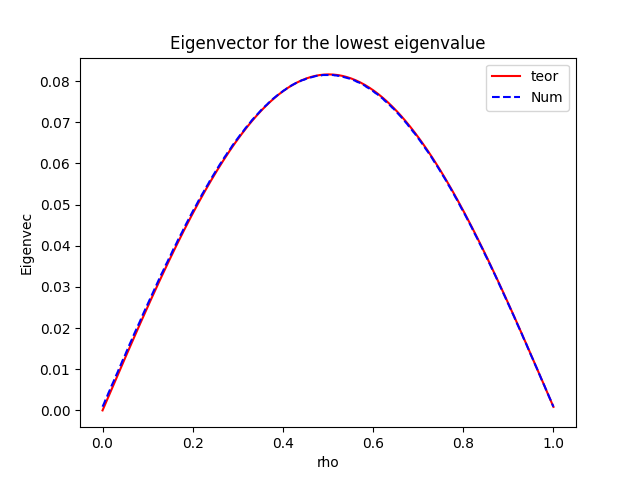
\includegraphics[width=\linewidth]{Egenvektorer1.png}
	\caption{Above we see a plot of the eigenvector for computed with the armadillo function $\text{eig\_sym}$ ($\text{Num}$), vs. the theoretical eigenvector (teor). This is for the buckling beam problem.}
	\label{fig:egen1}
\end{figure}

\begin{figure}[H]
	\centering
	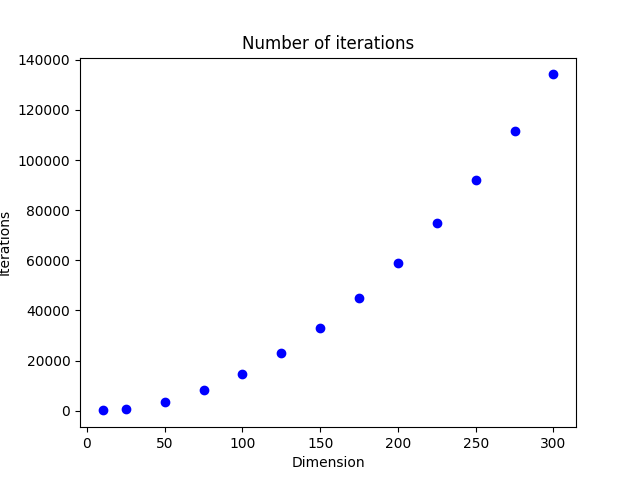
\includegraphics[width=\linewidth]{Iterasjoner.png}
	\caption{Above we have plotted the number of Jacobi rotations needed to make the non-diagonal elements essentially zero against the dimension of the matrix. (Buckling beam)}
	\label{fig:iter}
\end{figure}

\begin{figure}[H]
	\centering
	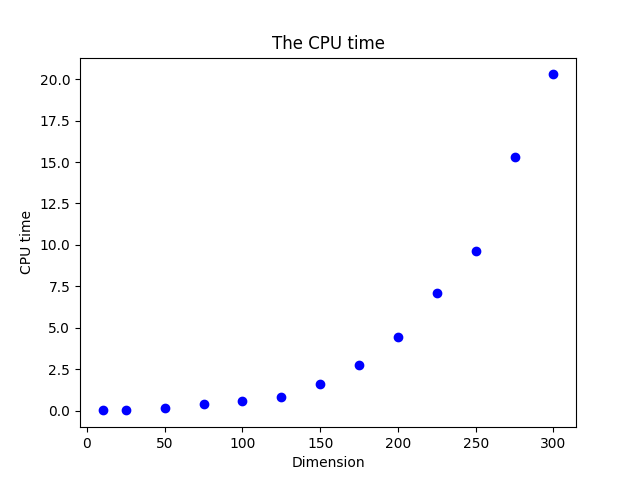
\includegraphics[width=\linewidth]{CPU_tid.png}
	\caption{Above we have plotted the CPU-time needed to make the non-diagonal elements essentially zero against the dimension of the matrix. (buckling beam)}
	\label{fig:CPU}
\end{figure}

For the buckling beam eigenvalue problem we were able to reproduce the eigenvalues with an accuracy of 1e-14 compared to the analytical values. For the case with quantum dots in three dimensions and one electron, we tried to find how many integration points was needed to reproduce the analytical results with four leading digits after the decimal point. For some reason, we weren't able to reproduce the analytical results with more than one leading digit after the decimal point. 

\begin{figure}[H]
	\centering
	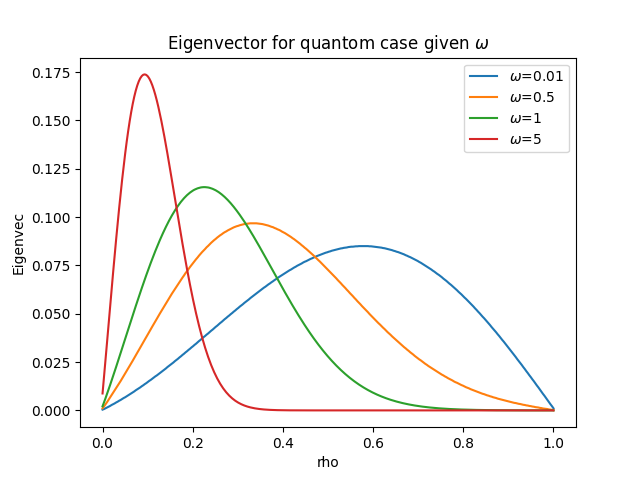
\includegraphics[width=\linewidth]{Egenvektorer_omega.png}
	\caption{Above we have plotted the eigenvectors for the quantum case with different values for $\omega$}
	\label{fig:omega}
\end{figure}

\section{Discussion}
From Figure (\ref{fig:egen1}) we can see that armadillo's function for computing eigenvectors seem to be very accurate which gives a good comparison tool when checking whether our code works. When looking at Figure (\ref{fig:iter}), it seems that the number of iterations against the dimension increases in a quadratic fashion. This might make sense, given the fact that the elements of a matrix also increases quadratic with the dimension. When looking at Figure (\ref{fig:CPU}), we can see that the CPU-time needed, seems to increase at an even faster rate. This might be due to the fact that at higher dimensions, the RAM might max out making the time needed per iteration higher for higher dimensions. As stated above, we weren't able to reproduce the analytical eigenvalues for the quantum case with one electron with more than one leading digit after the decimal point. We couldn't find the reason for why we couldn't, even though we tried different values for $\rho_{max}$ between 1 and 10, increasing the dimension, and adjusting the tolerance for the Jacobi algorithm. In addition, due to poor workflow management and a quite chaotic code we lost the data for the eigenvalues in both the buckling beam problem and the quantum case. We could've tried to reproduce them, but at this point we simply don't have the time for that. We believe that better planning and by using object oriented code, we could've avoided this specific problem. Finally, looking at Figure (\ref{fig:omega}) we see the eigenvectors for the quantum case using different values for $\omega$. Unfortunately we couldn't find the analytical solutions for the eigenvectors, so we are unable to tell if the eigenvectors we found represent the correct solutions.  

\section{Concluding remarks}
We were able to develop a code which solves the eigenvalue problem for the buckling beam problem with great accuracy, but encountered problems achieving the same accuracy for the quantum case. When solving eigenvalue problems with the Jacobi method, the number of iterations needed increases quadratic with the dimension of the matrix used. In other words, there is a trade-off between precision and time which needs to be taken into account when solving eigenvalue problems with the Jacobi algorithm. 
\bibliography{referanser}

\end{document}
